\documentclass[conference]{IEEEtran}
\usepackage[pdftex]{graphicx}
\usepackage[cmex10]{amsmath}
\interdisplaylinepenalty=2500
% \usepackage{algorithmic}
\usepackage{array}
\usepackage{mdwmath}
\usepackage{mdwtab}
\usepackage{eqparbox}
\usepackage[font=footnotesize]{subfig}
\usepackage{fixltx2e}
\usepackage{url}
\hyphenation{}

% additional packages and utility commands
\newcommand{\TODO}{\textbf{\color{red}TODO}}

\usepackage{minted}
\usepackage{flushend}

% while preparing, linenumbers come in handy
\usepackage{lineno}
\setlength\linenumbersep{1mm}
\linenumbers

% until we settle on the final name ;-)
\usepackage{xspace}
\newcommand{\NAME}{id-foo\xspace}

% http://tex.stackexchange.com/questions/299/how-to-get-long-texttt-sections-to-break
\newcommand*\justify{%
  \fontdimen2\font=0.4em% interword space
  \fontdimen3\font=0.2em% interword stretch
  \fontdimen4\font=0.1em% interword shrink
  \fontdimen7\font=0.1em% extra space
  \hyphenchar\font=`\-% allowing hyphenation
}

% http://en.wikibooks.org/wiki/LaTeX/Customizing_LaTeX
\newcommand{\ttt}[1]{\texttt{\justify{#1}}}

\usepackage{algpseudocode}
% custom Let command
\newcommand*\Let[2]{\State #1 $\gets$ #2}
\renewcommand{\algorithmicforall}{\textbf{for each}}
\let\ForEach\ForAll

\usepackage{listings}

\usepackage{tikz}

\begin{document}

% to avoid syntax error highlighting - e.g. foo's not js ;-)
\expandafter\def\csname PY@tok@err\endcsname{}

\title{
Introducing the \NAME Framework\\
for Efficient Intrusion Detection\\
in the Internet of Things
}

\author{\IEEEauthorblockN{Christophe Van Ginneken, Jef Maerien, Christophe
Huygens, Danny Hughes, Wouter Joosen}%
\IEEEauthorblockA{iMinds-DistriNet, KU Leuven\\
3001 Leuven, Belgium\\
\{firstname.lastname\}@cs.kuleuven.be}}

\maketitle

\begin{abstract}

Supporting multiple intrusion detection (ID) algorithms imposes significant
overhead on Internet of Things (IoT) devices. Fusion of the underlying
algorithms can alleviate this, yet, proves to be time-consuming, repetitive and
error-prone. To address this problem we introduce \NAME, a framework for the
development of efficient intrusion detection systems (IDS). It consists of a
domain specific language (DSL) that allows formally describing ID algorithms on
a functional level. A code generator then fuses these algorithms and produces
more optimally organised source code. This way, \NAME addresses the
heterogeneity of both the IoT and ID, as well as the limited resources of IoT
devices. A side-by-side comparison shows that generated code reduces memory
footprint, message passing overhead and execution time in comparison to a
straightforward sequential implementation of the same algorithms.

\end{abstract}

\section{Introduction}

% context

% IoT + threat

Along with its potential, the IoT also presents a significant threat: by
opening our smart homes \cite{aldrich2003smart} and personal data to all these
interconnected devices, we also open them to everyone who is able to break
these new, virtual locks, often without leaving a trace.

% classic networks: fw and central ids

In classic networks, firewalls focus on the outer perimeter of the network,
filtering unwanted packets and protecting the entire internal network. But
attacks on flaws in services can pass unnoticed. This is where intrusion
detection (ID) steps in: an ID probe monitors all traffic that passes through
the firewall, looking for patterns and optionally alerting the firewall if a
malicious pattern is detected \cite{denning1987intrusion}.

% manet: local ids -> localize -> limited resources

In mobile ad hoc networks (MANET), which make up an important part of the IoT,
it is not possible to have this single point in the network that can oversee
all traffic \cite{zhang2000intrusion, mishra2004intrusion}. If the outer
security perimeter diminishes, every device has to implement its own lines of
defence. Making the IDS a local service on each device requires resources,
which are another important constraint: IoT devices typically have limited
batteries, little processing power and memory is restricted to the bare minimum.

% gap analysis

Current developments in ID focus on programming frameworks to structure the
implementation of different algorithms \cite{valero2012di} and offer the
required basic functional components to implement actual algorithms
\cite{krontiris2008lidea}, but don't offer a way to optimise the usage of
resources. They also don't support systematic reuse to create different
configurations for different nodes or evolution in time.

% problem -> requirements for solution

The IoT is a heterogeneous environment, both in hardware and software.
Addressing this in a transparent and automated way is a key success factor for
any kind of development in this area. For a non-functional layer, such as ID,
this aspect becomes even more paramount.

A solution that supports the integration of multiple algorithms on IoT devices
needs to consider the impact on their resources. Different algorithms should be
merged to avoid accumulating their impact.

% my approach merged into ...
% scientific contribution

% 1. framework: language + code generator

The first contribution of this paper is a framework that enables the formal
description of ID algorithms on a functional level. An automated code
generation process produces corresponding source code, for a given platform and
configuration. This way, the framework addresses the heterogeneous nature of
both the IoT, as a hardware and software platform, and ID algorithms.

% 2. FCF to optimise

The second contribution introduces functional code fusion (FCF) as a generation
paradigm. FCF identifies common data and functions, and organises code in such
a way that redundant iterations, tests and computations are eliminated. Our
results show substantially improved memory usage, execution time and usage of
the wireless radio, reducing energy consumption.

% structure

The remainder of this paper proceeds as follows: section \ref{background}
details some of the ideas behind FCF and identifies the different aspects of
the problem space. Section \ref{design} describes the design we applied to
construct the framework, its domain specific language (DSL) and code generator.
Section \ref{evaluation} evaluates an implementation and application of the
framework. Section \ref{related} explores related work in the field of DSLs for
ID and code generation for the IoT. Finally, section \ref{conclusion}
summarises our findings, draws conclusions and identifies topics for future
work.

\section{Background}
\label{background}

The underlying problem addressed in this paper is of an economic nature: adding
ID doesn't add functionality, so its impact should be reduced as much as
possible.

In literature, many ID algorithm are described, but hardly any are implemented.
If implementations would be available, one would typically apply a pattern as
shown in listing \ref{alg:id-algo-application}.

\begin{figure}[H]
\captionof{lstlisting}{Sequential implementation of ID algorithms\label{alg:id-algo-application}}
\begin{algorithmic}[1]
  \Let{$msg$}{$network$} \Comment{all observed messages}
  \ForEach{$algorithm \in algorithms$}
    \State \Call{algorithm.progress\_message}{msg}
  \EndFor
  \State \dots
  \Comment{at a given interval}
  \ForEach{$algorithm \in algorithms$}
    \State \Call{algorithm.do\_housekeeping}{}
  \EndFor
\end{algorithmic}
\end{figure}

The implementations would be linked and called in a sequential way, when new
messages are observed on the network and at a regular interval to allow them to
do internal housekeeping. This includes processing the information extracted
from the network traffic, often in a statistical way.

This duality is a common design pattern of ID algorithms targeting MANETs. The
internals of the pattern reveal more common structures, as illustrated in
listing \ref{alg:id-algo-pattern}.

\begin{figure}[H]
\captionof{lstlisting}{ID Algorithm Pattern\label{alg:id-algo-pattern}}
\begin{algorithmic}[1]
  \Require{nodes, global storage for information about nodes}
  \Function{process\_message}{$msg$}
    \ForEach{$byte \in msg$} \label{alg:id-algo-pattern-loop1}
     \State \dots \Comment{analyse byte-sequences}
    \EndFor
    \Let{$nodes_x$}{value}  \Comment{optionally update node info}
    \State \Call{send}{$nodes_y$, ``info''} \Comment{optionally exchange info} \label{alg:id-algo-pattern-send1}
  \EndFunction
  \State
  \Function{do\_housekeeping}{}
    \ForEach{$node \in nodes$} \label{alg:id-algo-pattern-loop2} \label{alg:id-algo-pattern-common-data}
      \If{$node > \dots$} \Comment{validate recorded value}
        \State \dots \Comment{take actions}
        \State \Call{send}{$node$, ``info''} \Comment{e.g. communicate} \label{alg:id-algo-pattern-send2}
      \EndIf
    \EndFor
  \EndFunction
  \State
\end{algorithmic}
\end{figure}

The parts of interest here are the loops at lines
\ref{alg:id-algo-pattern-loop1} and \ref{alg:id-algo-pattern-loop2}, the common
\emph{nodes} data on line \ref{alg:id-algo-pattern-common-data} and the
interaction with the network at lines \ref{alg:id-algo-pattern-send1} and
\ref{alg:id-algo-pattern-send2}.

\subsection{Loops and Common Data}

Given several ID algorithms, that all execute the same parsing loop, over the
same byte stream, performing comparable operations to find similar patterns,
one would clearly benefit from combining these loops, avoiding redundant
reevaluation of the same byte patterns.

The same goes for common data. Each algorithm not only has to parse the same
message, it also has to store information about nodes within its own scope,
resulting in a lot of duplicated information in memory.

The only way to solve this, would be to change the provided implementation,
pulling up the loops over the message and the nodes to a level above the loop
over the algorithms. But this comes at a development cost. This cost typically
isn't a one-time cost, e.g. in case a new version of the algorithm is released,
or simply when a different set of algorithms is selected due to a changing risk
analysis. Finally, changing, or simply implementing the algorithms from
scratch, also holds the risk of making mistakes.

\subsection{Network Usage}

But there are hardly any implementations readily available. Probably the main
reason for this is the heterogeneity of the IoT. A prime example is the
\ttt{SEND} function. Different software stacks will have different application
programming interfaces (APIs) for accessing the network. Simple, macro-like
solutions can overcome this, but the dispersion of the calls to access the
network is causing the wireless radio to be on a lot more that one would hope
for.

A valid solution would try to combine messages in a single instance, reducing
the access to the network and even sharing some network overhead. The impact to
implement this manually will again outweigh the gain. An option would be to use
a software library, that provides a unified API for accessing the network and
collects individual calls and combines them in a single network message.

Besides the fact that all researchers would have to use the same library in a
consistent way, they would limit their operational scope to a single language,
serving only a fraction of the heterogeneous IoT.

\subsection{Situation Summary}

Starting from scratch allows optimising the implementation of an IDS, but
doesn't scale. Reusing existing implementations also doesn't help, due to the
far from optimal sequential execution of the algorithms and the redundant
storage of common data. Software libraries can solve many of the issues, but
only cover parts of the entire spectrum, due to their tie-in with languages and
frameworks.

\section{Design}
\label{design}

To bridge the gap between the research world and the heterogeneous IoT where
developers want to implement an actual IDS, while still respecting the limited
resources they have at their disposal, we introduce \NAME, a framework
consisting of a DSL, code generator and software library.

The DSL enables researchers to formally describe their ID algorithms, without
focusing on any specific language or platform. Given such formal descriptions
of ID algorithms, a code generator is now able to combine these, while avoiding
the sequential patterns/problems presented in listings
\ref{alg:id-algo-application} and \ref{alg:id-algo-pattern}. It can also target
different languages and platforms, while reusing a software library that
provides e.g. message parsing, network access wrapping,\dots

\subsection{DSL}

The DSL component of \NAME has two major goals and one minor: (1) allow the
description of ID algorithms in a formal way and (2) avoid that those
descriptions contain \emph{non-fusible} logic and/or data. Besides these (3)
the usability of the language is also taken into account.

The first goal is covered by the construction of the language itself. Given a
description of an ID algorithm using the DSL, the algorithm can be
unambiguously interpreted. The DSL borrows a lot of its syntax from C-like
languages, dropping only a small subset of its capabilities, but replacing
those with other higher-level constructs taken from object-oriented (OO)
languages, aspect-orientation,\dots

The most important omission from the C syntax are basic loops. Loops are very
generic and make it hard to identify if they deal with the same logic and/or
data. Fusing these loops across different algorithms is often non-trivial. In
\NAME's DSL, other constructs have been introduced to lift the definition of
these loops to a more functional level: scheduling and scoping of the execution
of functions, reacting to events and pattern matching are three examples that
allow describing the actual meaning of loops in stead of simply the loop
itself. It sometimes requires rethinking the reason behind a technical loop,
but often results in a much clearer description.

To deal with common data, the domain provides the notion of \emph{nodes}. As
most, if not all, ID algorithms targeting the IoT require some notion of the
other nodes or devices in the vicinity, the DSL makes this the primary
information carrier. All functional constructs, mentioned above, typically
operate on the collection of known nodes, or a functionally defined subset of
that. Each algorithm also has the possibility to \emph{extend} nodes, adding
its own properties needed for its execution.

Based on a C-like syntax the language is also very accessible. To further
nurture the usability, syntactic sugar from OO languages is also adopted.
Because not everything should be implemented in such a high-level language, it
also provides a way to \emph{import} external functionality. In the first place
this will include a standard library of functions that can be called, but it
can include any custom built software component. Finally it tries to limit the
need for type information and performs as much type inference as possible. As
it aims to be language that describes algorithms on a functional level it seeks
to safeguard its users from these \emph{technicalities}. The fact that the
opportunities of such a formal description include generation of code in a
variety of languages, each with possibly different types, also results the need
for a more functional approach to types.

Listing \ref{lst:heartbeat} illustrates some of the features mentioned above,
using a small but representative example of an algorithm: a heartbeat. Using a
heartbeat, nodes can broadcast a message at a regular interval, allowing other
nodes to monitor its availability. Missing heartbeats could indicate problems,
such as physical capturing of a certain node.

\lstinputlisting[
  float,
  basicstyle=\small\ttfamily,
  label=lst:heartbeat,
  caption=Heartbeat in \NAME
]{src/heartbeat.foo}

\subsection{Code Generator}

To convert the DSL based ID algorithms into production-ready code, we propose
the use of a code generator. Although many approaches here are applicable, like
template based text expansion, XSLT transformations or even using the
CodeDom\cite{dollard2004code}, we believe that for the level of functional
transformations that need to be performed, a richer model is required.

A semantic model \cite{fowler2010domain}, tied closely to the DSL itself, can
fulfil this role. Semantic transformations can now be applied to create a
code-oriented model, comparable to the idea of CodeDom. From there on,
syntactic transformations an emit actual source code. Figure
\ref{fig:code-generation} shows the overall procedure.

\begin{figure}[H]
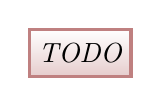
\begin{tikzpicture}[
    nonterminal/.style={
% The shape:
rectangle,
% The size:
      minimum size=6mm,
% The border:
      very thick,
      draw=red!50!black!50,
      % The filling:
top color=white,
bottom color=red!50!black!20, % and something else at the bottom % Font
font=\itshape
    }]
  \node [nonterminal] {TODO};
\end{tikzpicture}
\caption{Overview code generation process}
\label{fig:code-generation}
\end{figure}

\subsection{Semantic Model}

\TODO

Figure \ref{fig:meta-model} shows the meta-model of the the semantic model.

\begin{figure}[H]
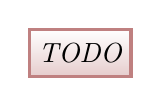
\begin{tikzpicture}[
    nonterminal/.style={
% The shape:
rectangle,
% The size:
      minimum size=6mm,
% The border:
      very thick,
      draw=red!50!black!50,
      % The filling:
top color=white,
bottom color=red!50!black!20, % and something else at the bottom % Font
font=\itshape
    }]
  \node [nonterminal] {TODO};
\end{tikzpicture}
\caption{Semantic Model Meta-Model}
\label{fig:meta-model}
\end{figure}

\subsection{Software Library}

\TODO

- incoming message parsing
- outgoing message grouping
- execution of schedules
- standard library: high-level conceptual functions (e.g. now(), sha1,...)

\section{Implementation and Evaluation}
\label{evaluation}

To evaluate the prototype we chose to use a system based on the Atmel
ATMEGA1284p micro-controller \cite{datasheet:atmega1284p} and the Digi XBee S2
ZigBee module \cite{manual:xbee}. To drive the hardware a minimalistic library
was used, wrapping the technical calls to the components in more easy to use
functions.

The reason for this at first sight unusual setup is simple: relying on basic
hardware and software allows us to validate that the generator is capable of
generating code even for the most basic environment available. Any step up,
both in hardware or software, would offer better and higher abstractions that
would make it easier to generate code for that situation. It shows that the
requirements of the generator towards the platform are minimal, don't rely on
advanced frameworks or operating systems and can therefore be applied in any
environment, targeting any platform.

For the evaluation we constructed a small meshed network consisting of three
devices, with only one device able to talk to both other devices, requiring
routing of messages through this device.

We started from a basic application that measures light intensity. The
application was written both manually and generated. On top of this baseline we
added two intrusion detection related algorithms: a heartbeat, that allows
nodes to validate each other's continuous presence, and a reputation-building
algorithm that checks if a parent node is cooperative and actually forwards
messages with a destination further down the
network\cite{ganeriwal2008reputation}.

Three criteria were evaluated: the image size of the resulting compiled code,
the network usage in number of frames and bytes and the time required to
perform once cycle of the event loop. These metrics were collected in four
situations: without ID algorithms, with a heartbeat, with reputation-tracking
and with both algorithms implemented.

In case of the manual implementation, both algorithms were constructed as
standalone modules and sequentially called from the base-application's event
loop. The code generator was provided with \NAME descriptions of the algorithms
and generated all four cases.

Before reviewing the results, it is very important to put these results in a
proper perspective. Comparing manually written code to generated code is no
exact science. One can always argue that the quality of the two code bases is
not comparable and that the manual code always can be improved. Still it might
be interesting to look at the numbers, given that both code bases are
constructed with the same intentions and practices. We believe we have achieved
this and have taken honest decisions while constructing the implementations,
making them comparable. Numerical analysis of the implementation offers us a
preliminary estimation of the effect of our proposed solution.

Tables \ref{tbl:manual} and \ref{tbl:generated} show the collected data
respectively for the manual and the generated implementation. The base case is
presented in absolute values, while the implementations with the added
algorithms are presented as relative values.

\begin{table}[H]
  \centering
  \begin{tabular}{lrrrr}
  \hline
      & base & heartbeat & reputation & both\\
  \hline
  size (bytes) & 10500 & 148\% & 127\% & 175\%\\
  frames & 20 & 255\% & 160\% & 315\%\\
  bytes & 476 & 406\% & 181\% & 487\%\\
  time ($\mu$s) & 48 & 196\% & 183\% & 310\%\\
  \hline
  \end{tabular}
  \caption{Results for the manual implementation.}
  \label{tbl:manual}
\end{table}

\begin{table}[H]
  \centering
  \begin{tabular}{lrrrr}
  \hline
         & base & heartbeat & reputation & both\\
  \hline
  size (bytes) & 10496 & 175\% & 156\% & 200\%\\
  frames & 20 & 245\% & 160\% & 275\%\\
  bytes & 476 & 399\% & 186\% & 454\%\\
  time ($\mu$s) & 48 & 252\% & 252\% & 288\%\\
  \hline
  \end{tabular}
  \caption{Results for the generated implementation.}
  \label{tbl:generated}
\end{table}

From these raw results, we learn that adding algorithms manually to the
base-application, results in a cumulative increase. The impact of both
algorithms is simply the sum of the impact of each algorithm by itself. In the
case of the time required to execute one cycle of the event loop, the total
time is even a bit higher than simply the sum.

In the case of the generated implementation, this no longer holds: although
that even the individual increases due to adding a single algorithm are higher
than in the manual case, the result for the implementation of both algorithms
is less than the sum of both. Here we clearly see the effect of reusing the
software library that comes with \NAME. The same goes for all other metrics.
Maybe most remarkable is the effect on the time of one event loop cycle: both
algorithms by itself add 150\% with respect to the base case, but when
combined, the impact hardly increases. Here we learn that the introduced
software library is responsible for the initial overhead, but it clearly pays
for itself when adding more algorithms.

Table \ref{tbl:summary} compares the two situations by subtracting the manual
case from the generated case, showing the impact of the code generation. A
relative value for the entire implementation with both algorithms is also
presented.

\begin{table}[H]
  \centering
  \begin{tabular}{lrrrrr}
  \hline
                & base & heartbeat & reputation & both  & result \\
  \hline
  size (bytes)  & -4    & 2822     & 3070       & 2664  & 115\%  \\
  frames        & 0     & -2       & 0          & -8    & 87\%   \\
  bytes         & 0     & -36      & 24         & -156  & 93\%   \\
  time ($\mu$s) & 0     & 27       & 33         & -11   & 93\%   \\
  \hline
  \end{tabular}
  \caption{Comparison of both implementations.}
  \label{tbl:summary}
\end{table}

When comparing the results of both implementations we first can conclude that
the generator produces exactly the same code for the base case. We couldn't
measure any real differences between both implementations.

Secondly, we see that the software library that comes with the generated code
adds to the size of the resulting image. But the cost is almost constant and is
relatively lower when algorithms are combined. With roughly 3KB of additional
overhead, or 15\% in this simple case, this impact is affordable.

From a functional point of view, the generated code lives up to the
expectations: both the number of frames as the bytes sent benefit from well
organised code and reuse of a common software library.

Finally we see that both algorithms by itself add an equal amount of time to
the processing of a single event loop cycle, but when combined, the event loop
is about 7\% faster compared to the manual case.

Without any effort to optimise the software library, nor leveraging knowledge
about the specific algorithms, this very basic generated code shows that the
proposed principles are not only theoretically feasible but actually result in
interesting improvements.

\section{Related Work}
\label{related}

IDS in WSN \cite{perrig2004security,mishra2004intrusion}

DSL \cite{fowler2010domain,mernik2005and}

DSL for WSN \cite{naumowicz2009prototyping,levis2004tinyscript}

DSL for IDS \cite{eckmann2002statl}

Code Generation for embedded systems/WSNs \cite{leupers2000code,marwedel2002code}

Code Optimization for embedded systems/WSNs \cite{panda2001data,naik2001software}

Code Generation for IDS \cite{charitakis2003code}

% manet: IDS algorithms -> coorporation, trust

More than in a classic network IDS, ID algorithms for MANETS operate with a
large degree of uncertainty. They often have to collaborate with other devices
in the network \cite{marchang2008collaborative,krontiris2009cooperative}, which
increases the level of uncertainty, because no other device can fully be
trusted. An IDS on an IoT device will be able to provide the services with
information about the reputation \cite{ganeriwal2008reputation} of other nodes
in the network.

\section{Conclusion and Future Work}
\label{conclusion}

theoretical gains are met in practice

explore more domains + implement corresponding DSLs for embedded systems

extract generic language as host for DSLs

Integration of applications with generated IDS allows actively and dynamically
responding to changes in the reputation of other nodes.

The services running on those devices can take advantage of these local
security layers. If the IDS detects a problem, the service can immediately
terminate the communication with the attacker, before it's actually abused.

\section*{Acknowledgements}

This research is partially funded by the Interuniversity Attraction Poles
Programme Belgian State, Belgian Science Policy, and by the Research Fund KU
Leuven. This research is partially funded by the EU FP7 project NESSoS. We
would like to thank the reviewers for their thoughtful and helpful comments
that enhanced the readability of this paper. Our gratitude and respect also
goes out to all members of the NES task force at KU Leuven/DistriNet for
creating the nurturing environment where these ideas could grow.

\bibliographystyle{IEEEtran}
\bibliography{literature/referenties}

\end{document}
